\documentclass[conference]{IEEEtran}
\IEEEoverridecommandlockouts
% The preceding line is only needed to identify funding in the first footnote. If that is unneeded, please comment it out.
\usepackage{cite}
\usepackage{amsmath,amssymb,amsfonts}
\usepackage{algorithmic}
\usepackage{graphicx}
\usepackage{textcomp}
\usepackage{xcolor}
\usepackage{blindtext}
\usepackage{hyperref}
\usepackage[spanish]{babel}
\def\BibTeX{{\rm B\kern-.05em{\sc i\kern-.025em b}\kern-.08em
    T\kern-.1667em\lower.7ex\hbox{E}\kern-.125emX}}
\begin{document}

\title{Implementación de enlaces punto a punto
}

\author{\IEEEauthorblockN{Germán Eduardo Castro Burgos}
\IEEEauthorblockA{\textit{Ingeniería de RF} \\
\textit{Universidad de Nariño}\\
Pasto, Colombia \\
$german\_castrob@hotmail.com$}
}
\maketitle

\section{Introducción}
La creciente necesidad de acceso a recursos informáticos ha traído consigo durante las últimas décadas,
un incipiente auge en el desarrollo de tecnologías que faciliten la implementación de sistemas de comunicaciones
en diversos escenarios rurales y urbanos. Las barreras topográficas existentes en algunas regiones, han determinado
en ocasiones la imposibilidad de brindar una solución factible para garantizar la conectividad de la región considerada, 
generando efectos adversos sobre la economía, educación y en general la calidad de vida de quienes habitan estas zonas.
Para mitigar los efectos descritos, diferentes alternativas tecnológicas se han propuesto considerando diversas metodologías
y medios de transmisión. Inicialmente los sistemas de comunicaciones basados en un medio físico (cable) contaban con capacidades
operativas significativamente superiores cuando su desempeño se contrastaba con el de sistema inalámbricos, que se veían limitados
por la cantidad de información que podía ser transferida luego de su despliegue. 

Con el incremento en la capacidad de procesamiento de sistemas embebidos y el surgimiento de nuevas técnicas de modulación de 
señales, la brecha entre sistemas inalámbricos y cableados se ha visto disminuida. Como resultado, la implementación de sistemas 
inalámbricos en áreas rurales o de dificil acceso es cada día mas frecuente. Los radioenlaces se presentan en dicho panorama, 
como una solución costo-efectiva para garantizar el acceso de comunidades aisladas a servicios de internet, y para establecer redes de 
comunicaciones multi propósito que contribuyen a garantizar la seguridad de la comunidad. El éxito de la solución propuesta estará 
relacionado con las consideraciones efectuadas durante la fase de diseño del enlace a emplear, siendo fundamentales la selección de los 
dispositivos que harán parte del sistema y la caracterización del enlace inalámbrico a partir de cálculos teóricos que requieren del uso 
de modelos de propagación y del reconocimiento de las regiones de Fresnel asociadas al escenario de trabajo. Este documento resume el procedimiento
llevado a cabo para la implementación de un enlace inalámbrico punto a punto, señalando las principales características de los elementos empleados,
las consideraciones previas a la implementación del enlace y un análisis comparativo de los resultados obtenidos frente a los pronósticos 
efectuados mediante la aplicación de las relaciones teóricas existentes para diferentes modelos de propagación.
\section{Descripción del experimento efectuado}
El ejercicio efectuado en busca de identificar las etapas que deben recorrerse para implementar de forma exitosa un radio enlace, tuvo como 
punto de partida la selección de los dispositivos a emplear para establecer la comunicación bi-direccional entre dos equipos terminales. Dado que el 
enlace propuesto corresponde en su configuración a un esquema punto a punto, en el que las comunicaciones se entablan exclusivamente entre dos
únicos nodos, es necesario implementar dos estaciones idénticas que permitan la transmisión de paquetes entre dos equipos de cómputo conectados
a cada extremo del enlace. Para identificar los efectos ocasionados sobre la potencia recibida en uno de los extremos del enlace, cuando se delimita
la primera zona de Fresnel, un obstáculo ha sido posicionado en el punto medio de la distancia que separa las estaciones transmisoras en busca de que
la señal reflejada sobre el mismo incremente el nivel de la potencia recibida. El escenario descrito puede apreciarse en la Figura @.
\begin{figure}
    \centering
          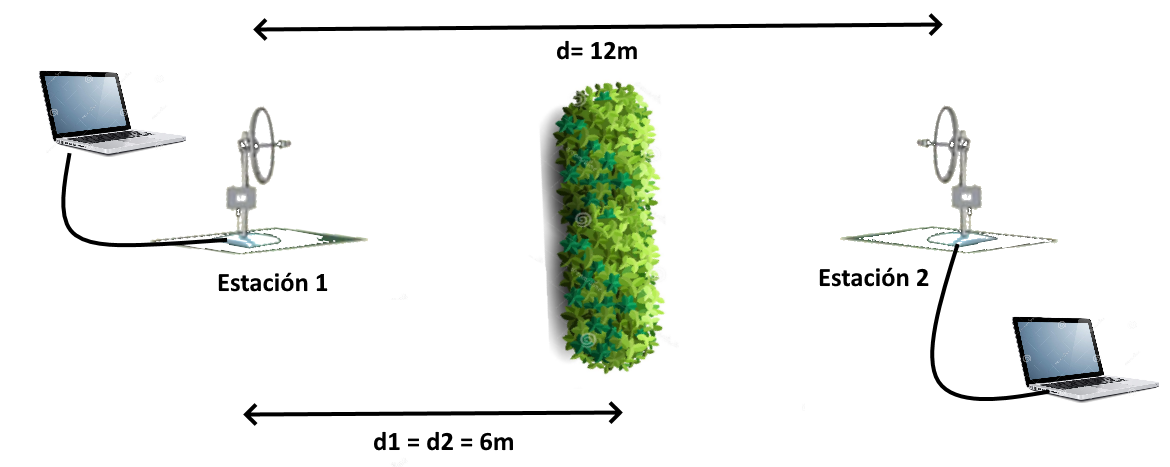
\includegraphics[width=0.47\textwidth]{Escenario.png}
        \caption{Antena tipo Rubber Duck HG2458-5RD-RSP.
        }
        \label{fig:Escenario}
\end{figure}
\subsection{Instrumentación empleada}
Cada una de las estaciones transmisoras está constituida por un conjunto antena-radio encargado de entablar comunicaciones con el nodo ubicado al 
otro extremo del enlace. El dispositivo principal de cada estación corresponde a un radio de referencia $Rocket M5$ del fabricante $Ubiquiti$. Según la 
información proporcionada por el fabricante, el equipo corresponde a una estación base empleada en la construcción de radio enlaces punto a punto y
punto a multi-punto. Puede alcanzar velocidades de hasta 150Mbps y ha sido diseñado en busca de facilitar la interacción con antenas de múltiple polarización.

La antena de referencia $AF-5G30-S45$ del fabricante $L-Com$ fue seleccionada para hacer parte de cada nodo del enlace. En su hoja de datos, el fabricante
describe al dispositivo como un equipo de alto desempeño empleado con frecuencia en conjunto con estaciones base de altas prestaciones, para establecer 
radio enlaces a largas distancias, cuando se requieren tasas de transferencia considerables, dadas su alta ganancia y patrón de radiación altamente directivo. 
La Figura @ muestra una imagen de los equipos empleados mientras en el Cuadro ! han sido consignados los valores correspondiente a sus pricipales parámetros
operativos. Entre los accesorios adicionales empleados durante a ejecución de la práctica pueden citarse un par de trípodes para topografía, cables de red de
diversas longitudes, fuentes de poder tipo $\textit{Power over ethernet (PoE)}$, adaptadores para conexión de las antenas y dos computadores portátiles que hicieron 
las veces de estaciones terminales.  
\begin{figure}
    \centering
          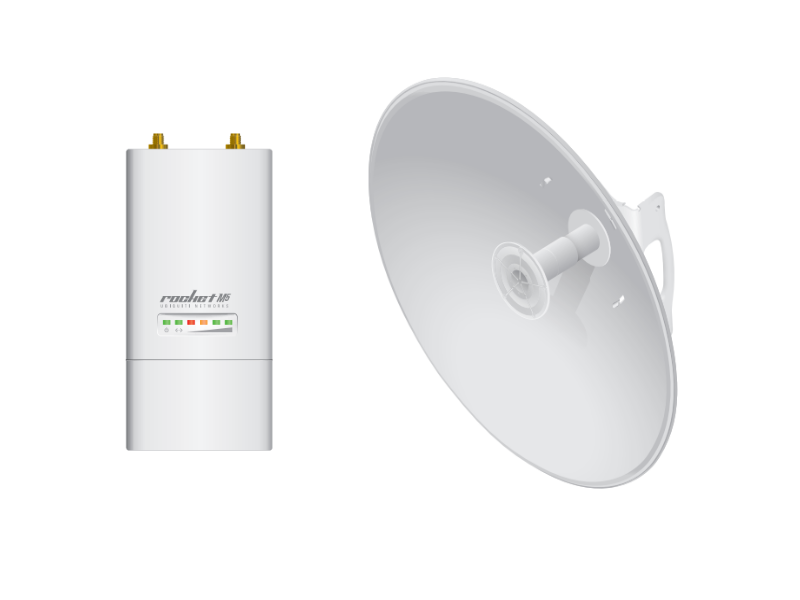
\includegraphics[width=0.4\textwidth]{Equipos.png}
        \caption{Antena tipo Rubber Duck HG2458-5RD-RSP.
        }
        \label{fig:Equipos}
\end{figure}
\begin{table}[!hbt]
    \begin{center}
        \begin{tabular}{ l  l }
            \hline
            \multicolumn{2}{c}{\textbf{Estación Base Rocket M5}} \\
            \hline
            \hline
            \textbf{Parámetro} & \textbf{Valor}\\
            \hline
            Modos de Operación & Punto de acceso, Estación\\
            Interfaz de Red & 10/100Mbps \\
            Puertos de Conexión RF & 2 X RP-SMA \\
            Frecuencia de Operación & 5150MHz-5875MHz \\
            Potencia Máxima Tx & 27dBm\\
            Protocolos soportados & 802.11a, 802.11n/airMax \\
            \hline
            \multicolumn{2}{c}{\textbf{Antena AF-5G30-S45}} \\
            \hline
            \hline
            \textbf{Parámetro} & \textbf{Valor}\\
            \hline
            Frecuencias de Operación & 4900MHz-5900MHz \\
            Polarización & Dual (+$45^\circ$), -$45^\circ$\\
            Ganancia & 4.9GHz: 26dBi \\
                     & 5GHz-5.9GHz: 30dBi \\
            Diámetro & 650 mm \\
            Ángulo Radiación +$45^\circ$  & $5.8^\circ$ \\
            Ángulo Radiación -$45^\circ$  & $5.8^\circ$\\
            \hline\\
        \end{tabular}
    \caption[]{Parámetros operativos antena HG2458-5RD-RSP}
    \label{Cuadro:1}
    \end{center}
\end{table}
\subsection{Configuración de las Estaciones Base}
Para implementar el radio enlace propuesto, cada una de las estaciones base ubicadas en los nodos extremos del 
mismo debe ser configurada siguiendo la arquitectura correspondiente a una conexión punto a punto. Para alcanzar 
tal fin, uno de los $RocketM5$ debe ser configurado en modo punto de acceso en busca de que su similar, ubicado en el
nodo remoto opere en modo estación a fin de fijar la señal transmitida por el punto de acceso. Dicha señal debe estar
identificada por una etiqueta que la diferencie de otras transmisiones efectuadas sobre la misma banda de frecuencias 
seleccionada. La configuración descrita es llevada a cabo empleando la interfaz web disponible en cada uno de los equipos,
a partir de la dirección IP que les ha sido asignada. Estaciones base y computadores portátiles emplean la dirección de red 
clase C $\textit{192.168.1.0}$ de forma tal que el punto de acceso corresponde a la dirección $\textit{192.168.1.20}$, la estación remota a
la dirección $\textit{192.168.1.21}$ y los equipos terminales de estación base y remota a las direcciones $\textit{192.168.1.24}$ y $\textit{192.168.1.25}$
respectivamente. Puesto que la ganancia de las antenas seleccionadas para la implementación del enlace corresponde a valores
considerablemente altos (30dBi), la potencia transmitida por la estación base se limitó a -4dBm considerando la corta 
distancia (12m) que la señal emitida debe recorrer para alcanzar a la estación remota. Finalmente, el canal seleccionado 
para la ejecución de la transmisión corresponde al constituido por las frecuencias comprendidas entre los 5175MHz y los 5215MHz, 
siendo la frecuencia central del mismo igual a 5195MHz.
\section{Metodología de Medición}
Una vez realizada la configuración requerida por cada uno de los componentes del radio enlace, las antenas correspondientes a 
estación base y estación remota fueron orientadas de forma tal que la potencia recibida en cada nodo alcanzara su valor máximo. El 
procedimiento fue repetido para variaciones en la altura de montaje de las antenas en busca del valor máximo de potencia recibida. 
Establecida la disposición óptima para la operación, se realizaron variaciones paulatinas sobre la altura de la antena del punto de acceso
registrando los valores de potencia recibida suministrados por el radio configurado como punto de acceso, que corresponden a las polarizaciones vertical y horizontal 
y al valor promedio generado a partir de las mismas. La altura de la antena correspondiente a la estación remota permaneció constante en 1.40m en tanto
que para el obstáculo ubicado en el punto medio de la distancia de separación entre estaciones la altura registrada correspondió a los 1.17m.
\section{Resultados Obtenidos}
\subsection{Valores obtenidos para potencia recibida}
Concluido el plan de mediciones propuesto se establecieron tres conjuntos de 15 parejas de datos altura-potencia recibida derivados de la información suministrada
por la estación base. Los valores de potencia recibida analizados corresponden a las polarizaciones vertical y horizontal y a la potencia
promedio calculada por el radio que hace parte de la estación base. A partir de dichos conjuntos, pueden construirse gráficas de la potencia recibida en función de la 
altura de la antena transmisora para cada caso, según se aprecia en la Figura @. Los resultados observados serán empleados para contrastar los valores de potencia 
recibida generados a partir de cálculos teóricos que emplean el modelo de propagación en espacio libre y el modelo de propagación de Barnett-Vignants.
\begin{figure}
    \centering
          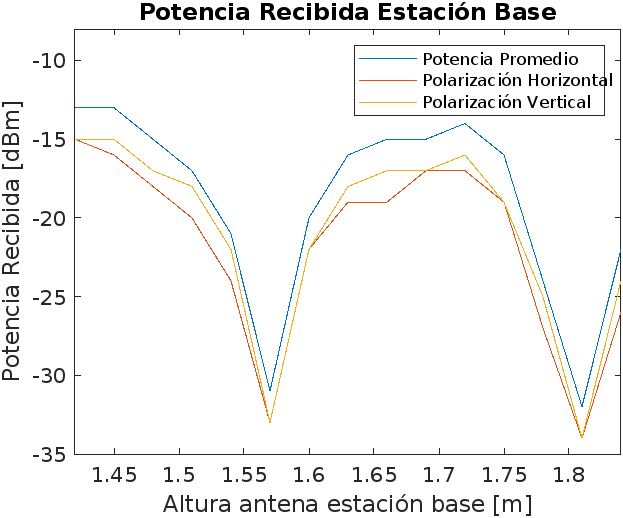
\includegraphics[width=0.4\textwidth]{Potencias.png}
        \caption{Antena tipo Rubber Duck HG2458-5RD-RSP.
        }
        \label{fig:Potencias}
\end{figure}
\subsection{Análisis de la zona de Fresnel}
Considerando las condiciones operativas del radio enlace implementado, es posible efectuar la caracterización teórica de la 
zona de Fresnel existente como resultado de dicho despliegue. La zona de Fresnel puede ser definida como una región cercana a la 
linea de vista apreciable entre los nodos de un radio enlace que debe encontrarse libre de obstáculos en busca de prevenir los efectos negativos
generados sobre la señal en el receptor como consecuencia de fenómenos de multi trayectoria. Su geometría está definida por una serie de elipses 
posicionadas al rededor de la línea de vista del enlace que establecen la distancia adicional recorrida por los componentes de la señal
que se han difractado en su recorrido. Existen por lo tanto diversas zonas de Fresnel aunque en la mayoría de circunstancias el análisis 
sobre el comportamiento de la señal se centra sobre las tres primeras.  En la primera zona de Fresnel las componentes difractadas de la señal
original contribuyen a incrementar la potencia recibida en los extremos del enlace. 

La caracterización de la zona de Fresnel corresponde al proceso mediante el cual se determina la altura adicional $r_1$ que debe tener la línea de vista
frente a la altura de un obstáculo determinado $h$ para un radio enlace establecido, según puede apreciarse en la Figura @. Para determinar el valor de $r_1$ la 
relación expresada en ! es aplicada, siendo $\lambda$ la longitud de onda correspondiente a la frecuencia de operación y $d_1$ y $d_2$ las distancias existentes
entre los extremos del enlace y el obstáculo analizado.
\begin{figure}
    \centering
          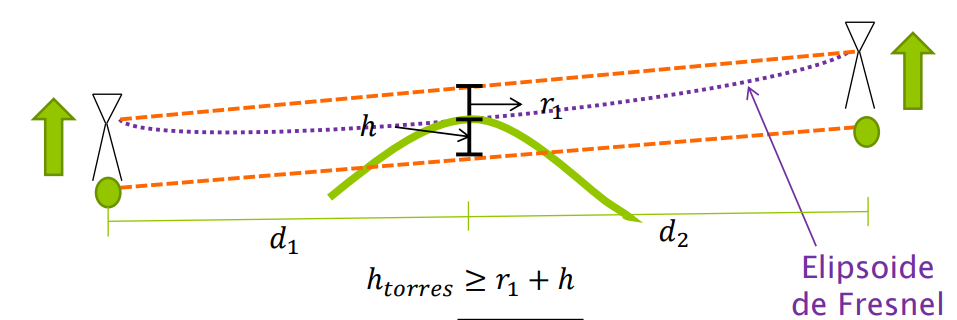
\includegraphics[width=0.47\textwidth]{Fresnel.png}
        \caption{Antena tipo Rubber Duck HG2458-5RD-RSP.
        }
        \label{fig:Fresnel}
\end{figure}
\begin{equation}
    \label{eq:Eq1}
    \begin{aligned}
        &r_{1} = \sqrt[2]{\lambda\frac{d_1d_2}{d_1+d_2}}\\
        &r_{1} = \textit{Radio primera zona de Fresnel}\\
        &d_{1} = \textit{Distancia estación 1 a obstáculo}\\
        &d_{2} = \textit{Distancia estación 2 a obstáculo}\\
        &\lambda = \textit{Longitud de onda para la frecuencia de operación}\\
    \end{aligned}
\end{equation}
Aplicando los valores correspondientes al enlace constituido, es posible determinar el valor de $r_1$ siguiendo el procedimiento
señalado en !.
\begin{equation}
    \label{eq:Eq2}
    \begin{aligned}
        &d_1=d_2=6[m]\\
        &f_0 = 5195[MHz]\\
        &c = 2.998*10^{8}[m/s]\\
        &\lambda = \frac{c}{f_0}=0.0577[m]\\
        &r_{1} = \sqrt[2]{\lambda\frac{d_1d_2}{d_1+d_2}}\\
        &r_{1} = \sqrt[2]{0.0577[m]\frac{6[m]*6[m]}{6[m]+6[m]}}\\
        &r_{1} = 0.4161[m]\\
    \end{aligned}
\end{equation}
Considerando que la altura del obstáculo existente en el punto medio del trayecto cubierto por el radio enlace se estableció en $1.17[m]$, siguiendo 
los planteamientos establecidos durante la descripción de la zona de Fresnel es posible afirmar que la altura de las torres de transmisión y recepción 
puede ser determinada siguiendo las indicaciones especificadas en !. Las antenas empleadas para la implementación del enlace propuesto deben ubicarse entonces
a una altura igual a $1.816[m]$ para cumplir con la restricción impuesta por la primera zona de Fresnel.
\begin{equation}
    \label{eq:Eq3}
    \begin{aligned}
        &h =1.17[m]\\
        &r_1 = 0.4161[m]\\
        &h_{torre} = h+r_{1}=1.816[m]\\
    \end{aligned}
\end{equation}
Haciendo uso de los procedimientos descritos es posible establecer el radio de la primera zona de Fresnel a lo
largo de la distancia correspondiente al enlace, de forma tal que el valor del mismo sea establecido en función 
de la distancia a la que un obstáculo de prueba pueda ser ubicado. La Figura @ muestra el resultado alcanzado para 
tal función sobre un enlace que abarca 12m de separación y opera a una frecuencia de 5195MHz.
\begin{figure}
    \centering
          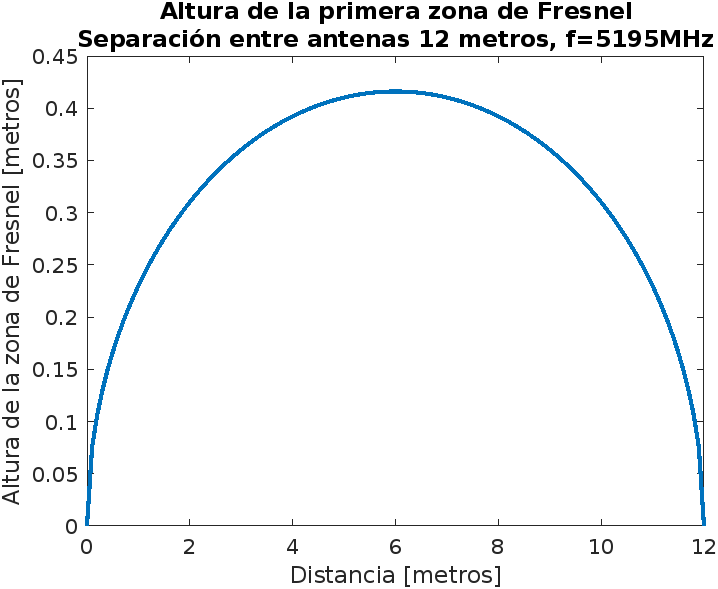
\includegraphics[width=0.45\textwidth]{Altura_Fresnel.png}
        \caption{Antena tipo Rubber Duck HG2458-5RD-RSP.
        }
        \label{fig:Altura_Fresnel}
\end{figure}
\section{Comparación de los resultados obtenidos con los modelos de propagación considerados}
Para determinar el nivel de ajuste de los datos recolectados frente a las estimaciones efectuadas a partir de 
los conceptos teóricos, se han seleccionado los modelos de propagación en el espacio libre y de Barnett-Vignants
para determinar los niveles de potencia recibida que se espera observar una vez el enlace implementado entre en operación.
El modelo de propagación en espacio libre determina el nivel de potencia recibida en función de la distancia y la 
frecuencia de operación considerando a la vez los valores correspondientes a la potencia transmitida y a las ganancias
de transmisión y recepción, según se muestra en !. 
\begin{equation}
    \label{eq:Eq4}
    \begin{aligned}
        &P_{rx}[dBm] = P_{tx} + G_{tx} + G_{rx} - L_{fs}\\
        &L_{fs}[dB] = 32.45+20logd[Km]+20logf[MHz]\\
        &P_{rx} = \textit{Potencia recibida}\\
        &P_{tx} = \textit{Potencia transmitida}\\
        &G_{tx} = \textit{Ganancia de transmisión}\\
        &G_{rx} = \textit{Ganancia de recepción}\\
        &L_{fs} = \textit{Pérdidas en el espacio libre}\\
        &d = \textit{Distancia hasta el punto de transmisión}\\
        &f = \textit{Frecuencia de operación}\\
    \end{aligned}
\end{equation}
Empleando los datos correspondientes al enlace establecido, es posible determinar el valor ideal para la potencia recibida 
a partir del procedimiento indicado en !. Empleando la información descrita se establece un valor para la pérdidas de espacio libre
igual a $68.3453[dB]$ y un estimado para la potencia recibida ideal igual a $-12.3453[dBm]$.
\begin{equation}
    \label{eq:Eq5}
    \begin{aligned}
        &d = 12[m] = 0.012[Km]\\
        &f = 5195[MHz]\\
        &P_{tx} = -4[dBm]\\
        &G_{tx} = G_{rx} = 30[dBi]\\
        &L_{fs} = 32.45+20log(0.012[Km])+20log(5195[MHz])\\
        &L_{fs} = 68.3453[dB]\\
        &P_{rx} = -4[dBm] + 30[dBi] + 30[dBi] - 68.3453[dB]\\
        &P_{rx} = -12.3453[dBm]
    \end{aligned}
\end{equation}
El modelo de Barnett-Vignants por su parte, agrega un margen de desvanecimiento sobre el valor ideal de
la potencia recibida considerando las características del terreno y las condiciones meteorológicas de lugar
de montaje, mediante un coeficiente denominado $C$. El margen depende también del grado de disponibilidad deseado 
para el enlace establecido, parámetro que se representa con la letra $R$ en la relación indicada en !. 
\begin{equation}
    \label{eq:Eq6}
    \begin{aligned}
        &M_{f}[dB] = 30logd[Km] + 10log6Cf[GHz]\\
        & - 10log(1-R) - 70\\
        &P_{rx}[dBm] = P_{tx} + G_{tx} + G_{rx} - L_{fs} - M_{f}\\
        &d = \textit{Distancia hasta el punto de transmisión}\\
        &f = \textit{Frecuencia de operación}\\
        &C = \textit{Factor condiciones ambientales}\\
        &R = \textit{Disponibilidad del enlace}\\
        &M_{f} = \textit{Margen de desvanecimiento}\\
        &P_{rx} = \textit{Potencia recibida}\\
        &P_{tx} = \textit{Potencia transmitida}\\
        &G_{tx} = \textit{Ganancia de transmisión}\\
        &G_{rx} = \textit{Ganancia de recepción}\\
        &L_{fs} = \textit{Pérdidas en el espacio libre}\\
    \end{aligned}
\end{equation}
Una vez más, empleando los valores correspondientes a cada parámetro requerido es posible determinar el valor
para el margen de desvanecimiento que permite establecer el valor final para la potencia recibida estimada. Considerando
que el lugar seleccionado para el despliegue del montaje cuenta con características meteorológicas del entorno urbano y
que el terreno no describe pendientes pronunciadas ni vegetación significativa, el coeficiente $C$ puede tomar el valor 1.
En cuanto a la disponibilidad del enlace, se establece que dada la baja distancia a cubrir el valor de $R$ debe aproximarse 
a 1 en busca de señalar que la comunicación debe efectuarse de forma permanente. Establecidos lo valores necesarios, el procedimiento 
llevado a cabo para determinar el margen del desvanecimiento y estimar el valor de la potencia recibida se muestra en !.
\begin{equation}
    \label{eq:Eq7}
    \begin{aligned}
        &C = 1\\
        &R = 0.999\\
        &d = 12[m] = 0.012[Km]\\
        &f = 5195[MHz]\\
        &P_{tx} = -4[dBm]\\
        &G_{tx} = G_{rx} = 30[dBi]\\
        &L_{fs} = 32.45+20log(0.012[Km])+20log(5195[MHz])\\
        &L_{fs} = 68.3453[dB]\\
        &M_{f} = 30log(0.012[Km]) + 10log(6*1*5.195[GHz])\\
        & - 10log(1-0.999) - 70\\
        &M_{f} = 7.3128[dB]\\
        &P_{rx} = -4[dBm] + 30[dBi] + 30[dBi] - 68.3453[dB]\\
        & - 7.3128[dB]\\
        &P_{rx} = -19.6581[dBm]
    \end{aligned}
\end{equation}
Concluida la caracterización del enlace, los resultados derivados de la misma empleando los modelos de 
propagación en el espacio libre y de Barnett-Vignants pueden resumirse según se indica en el Cuadro !.
\begin{table}[!hbt]
    \begin{center}
        \begin{tabular}{ l  l }
            \hline
            \hline
            \textbf{Parámetro} & \textbf{Valor}\\
            \hline
            Potencia transmitida & -4 dBm \\
            Ganancia de las antenas & +30 dBi\\
            Pérdidas de espacio Libre & -68.3453 dB \\
            \textbf{Potencia recibida ideal} & \textbf{-12.3453 dBm} \\
            Margen de desvanecimiento & -7.3128 dB \\
            \textbf{Potencia recibida estimada}  & \textbf{-19.6581 dBm}\\
            \hline
            \hline\\
        \end{tabular}
    \caption[]{Parámetros operativos antena HG2458-06DPU2}
    \label{Cuadro:3}
    \end{center}
\end{table}
Finalmente, los modelos descritos pueden ser empleados para establecer teóricamente el comportamiento de la potencia 
recibida a lo largo del enlace implementado. Las funciones que describen dicho comportamiento en función de la distancia 
de medición pueden apreciarse en la Figura @. 
\begin{figure}
    \centering
          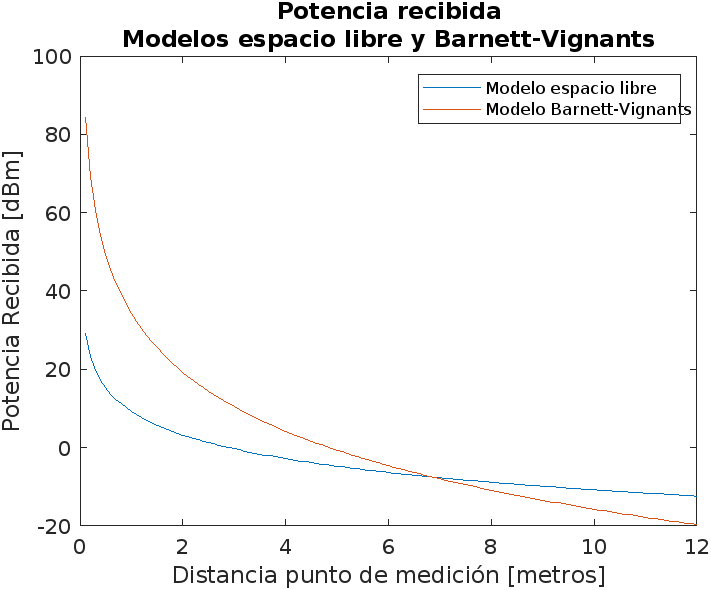
\includegraphics[width=0.45\textwidth]{Potencia_Modelos.png}
        \caption{Antena tipo Rubber Duck HG2458-5RD-RSP.
        }
        \label{fig:Potencia_Modelos}
\end{figure}
\section{Conclusiones}
\end{document}